\subsection{Taxi Event Distribution}
\label{section_taxi_denstiy_distribution}

To validate \emph{Claim~2}, we quantitatively analyze vehicles density in one hour periods. By dividing the whole network into $100 \times 100$ grids, taxi density distributions for load and drop event are computed in each cell. Fig.~\ref{figure_taxi_density_for_one_hour} shows the load/drop events distributions in three time periods. In the morning one, people begin to get out from home, so the load-event distribution is more even than that of drop-event. This phenomenon may be caused by the load-event spots are mainly at homes of the citizens, while the drop-event spots tend to gather together at workplaces, railway stations or scenic spots. Besides, in the evening time period, the dispersion of load-event is of lower degree than that of drop-event, for people coming home at that time. Overall, the amount of loading/dropping passengers in each cell shows geographic features: the distribution is uneven, and the difference between load/drop-event distributions illustrates the load/drop-event regions are different. All of these support \emph{Claim 2}.

%\begin{figure}[!h]
%\centering
%\vspace{0.in}
%\subfigure[$load,7:00-8:00$]{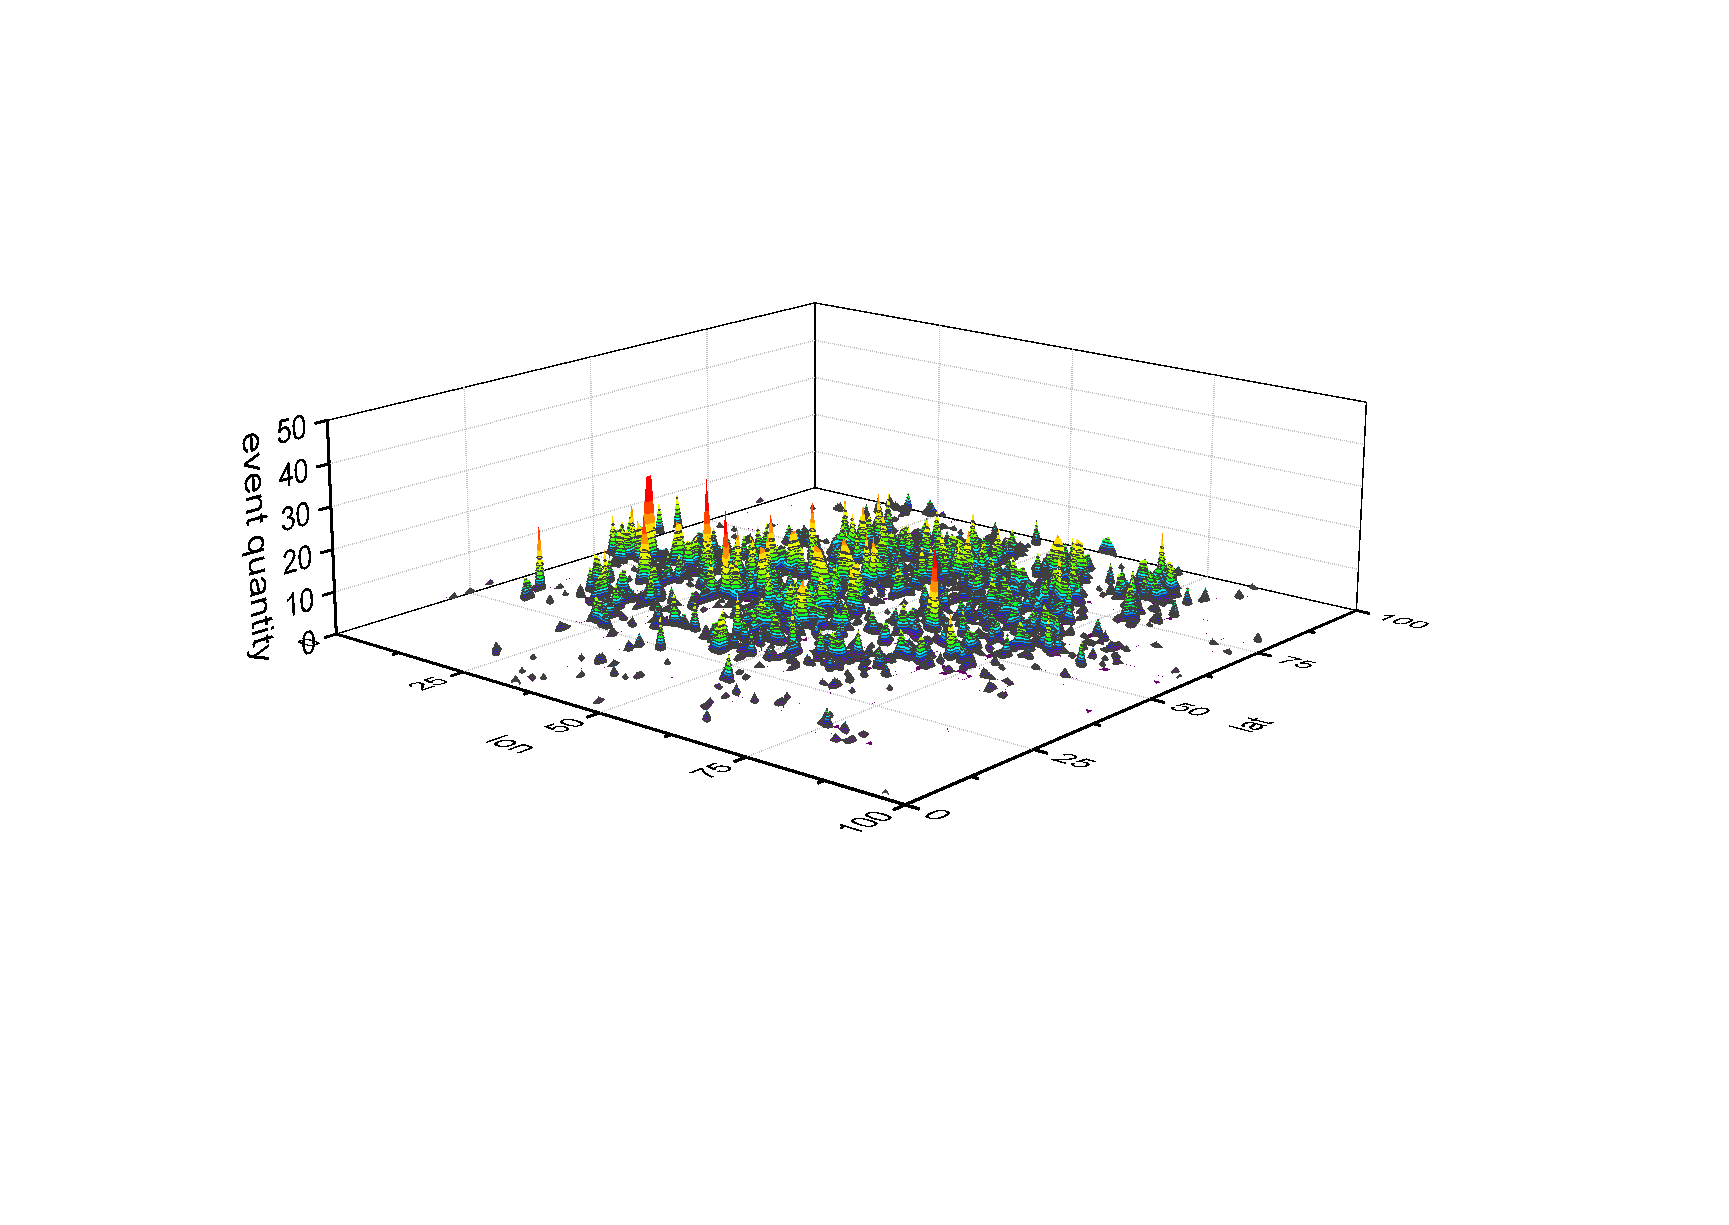
\includegraphics[width=0.23\textwidth]{figures_201103/events_dis/Graph4.eps}}
%\vspace{-0.14in}
%\subfigure[$drop,7:00-8:00$]{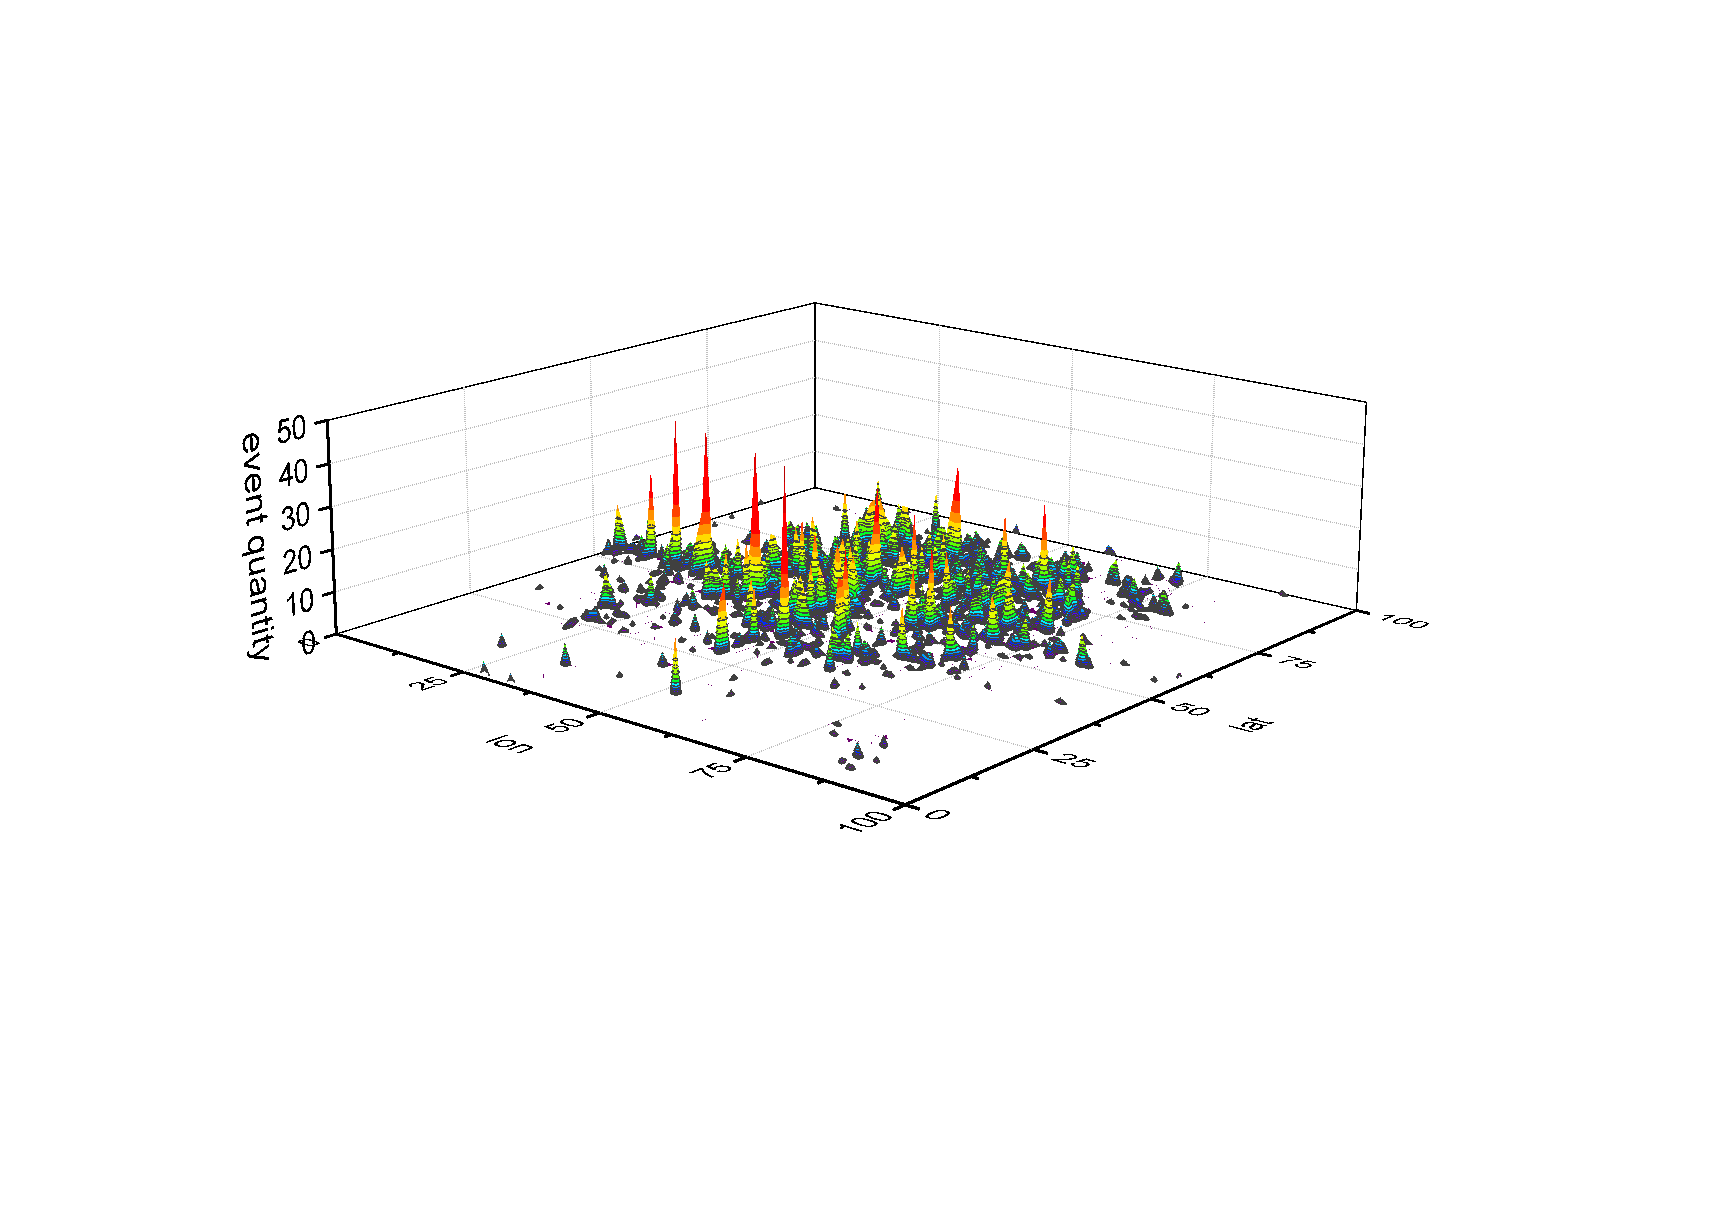
\includegraphics[width=0.23\textwidth]{figures_201103/events_dis/Graph1.eps}}
%\vspace{-0.14in}
%\subfigure[$load,12:00-13:00$]{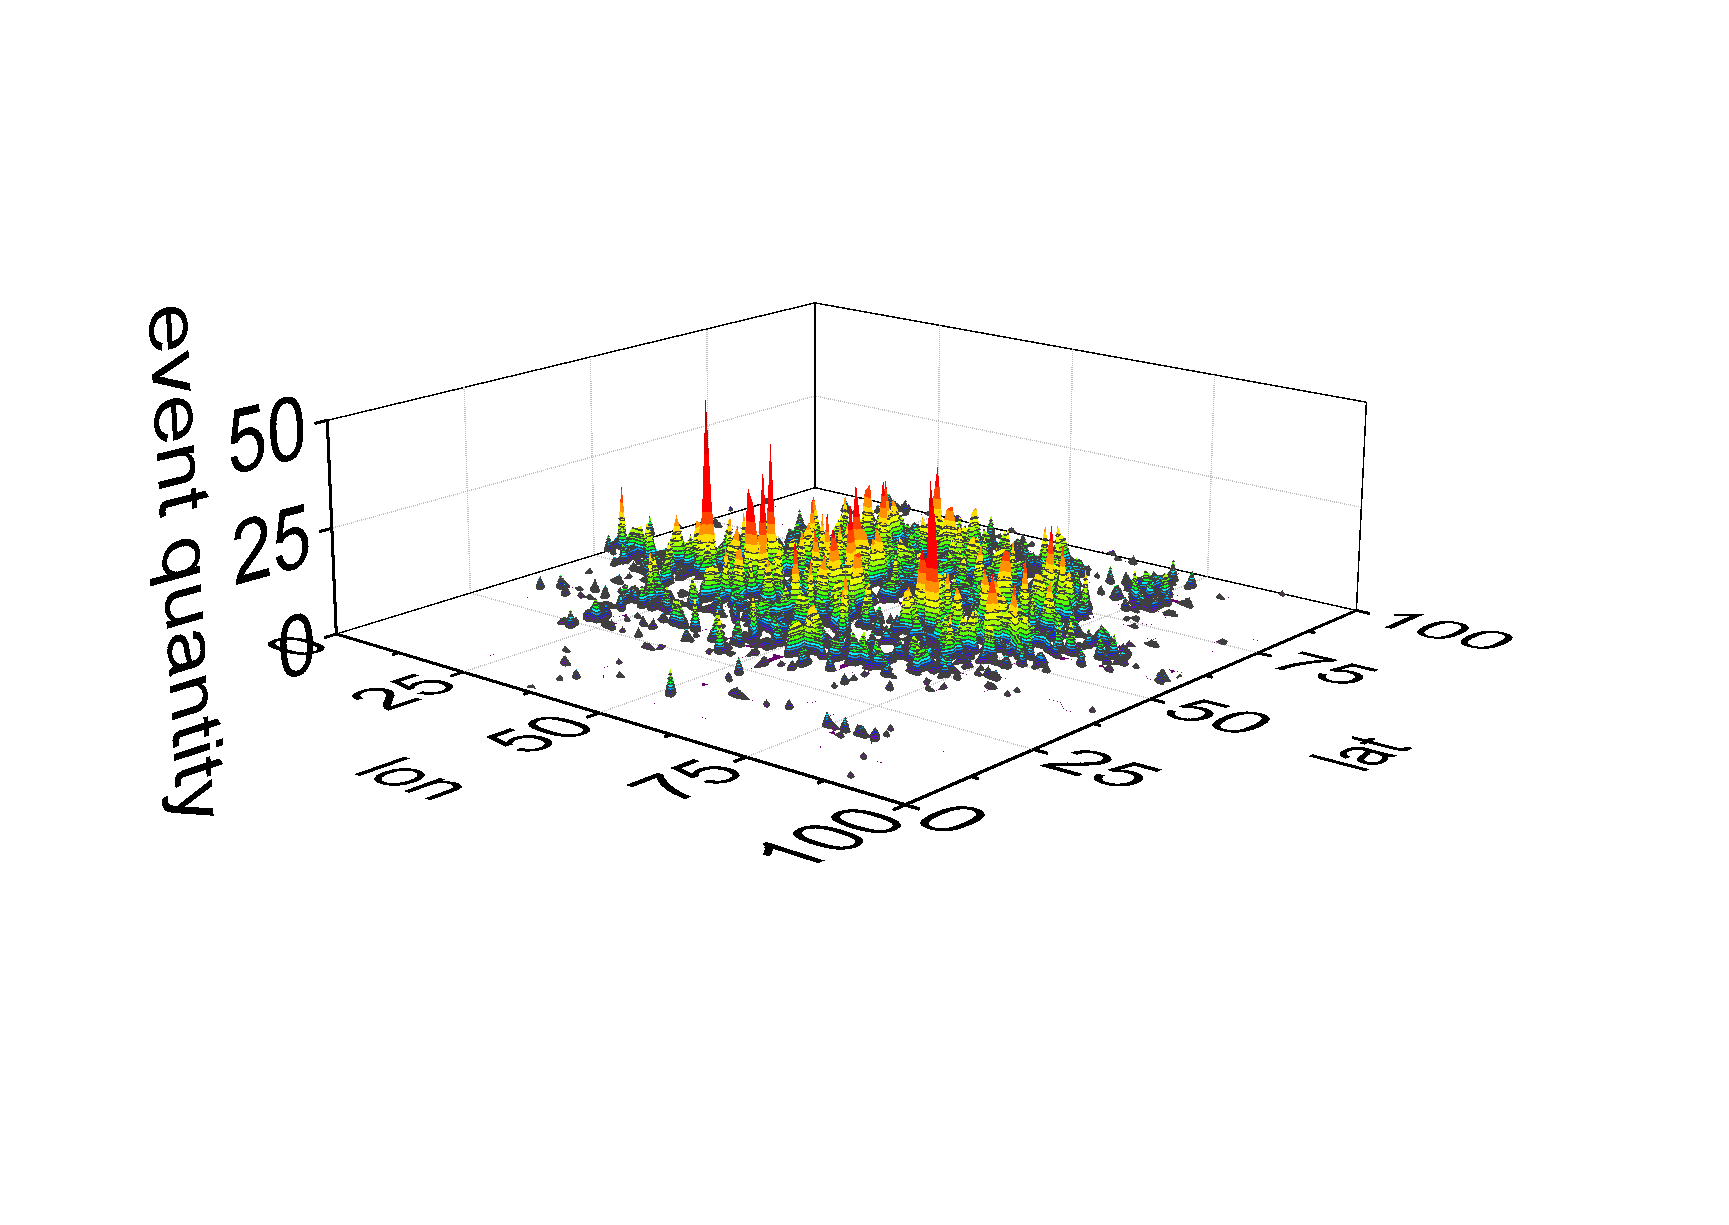
\includegraphics[width=0.23\textwidth]{figures_201103/events_dis/Graph5.eps}}
%\vspace{-0.14in}
%\subfigure[$drop,12:00-13:00$]{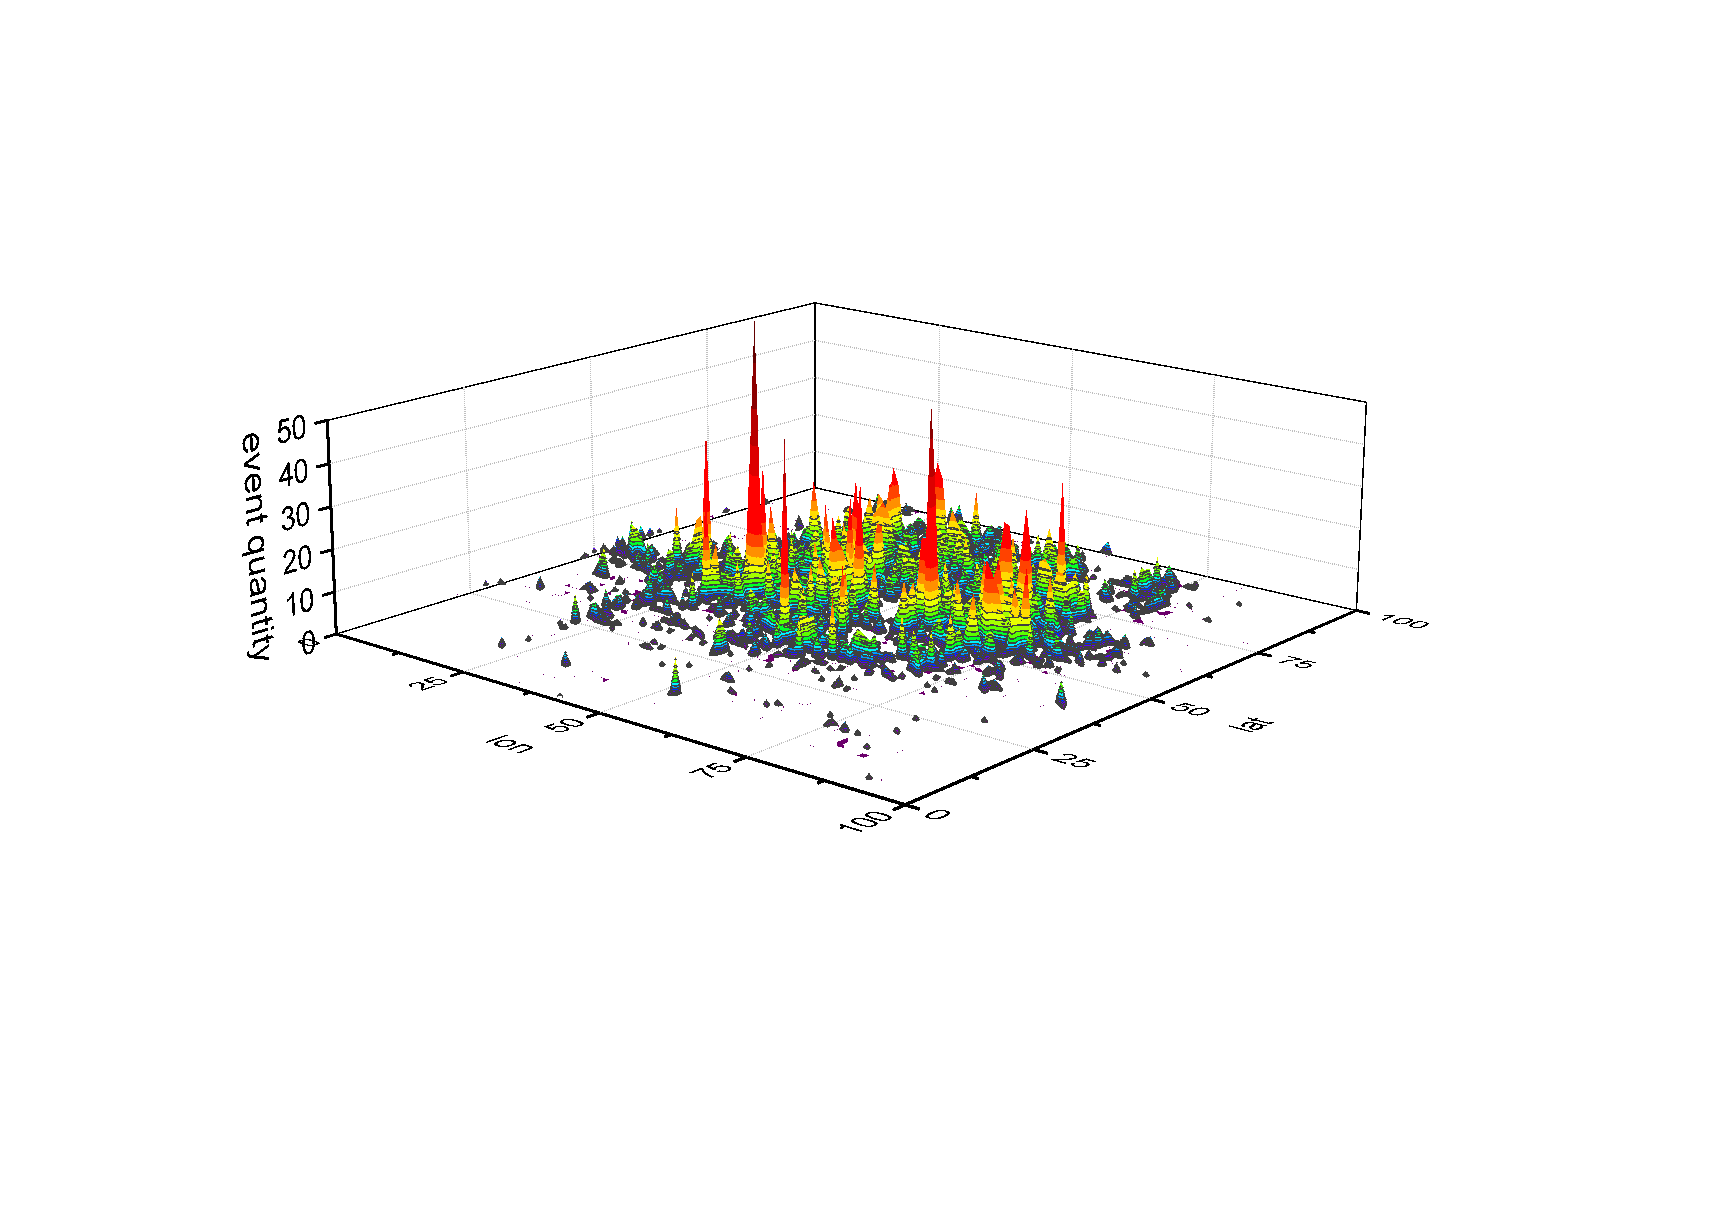
\includegraphics[width=0.23\textwidth]{figures_201103/events_dis/Graph2.eps}}
%\vspace{-.14in}
%\subfigure[$load,17:00-18:00$]{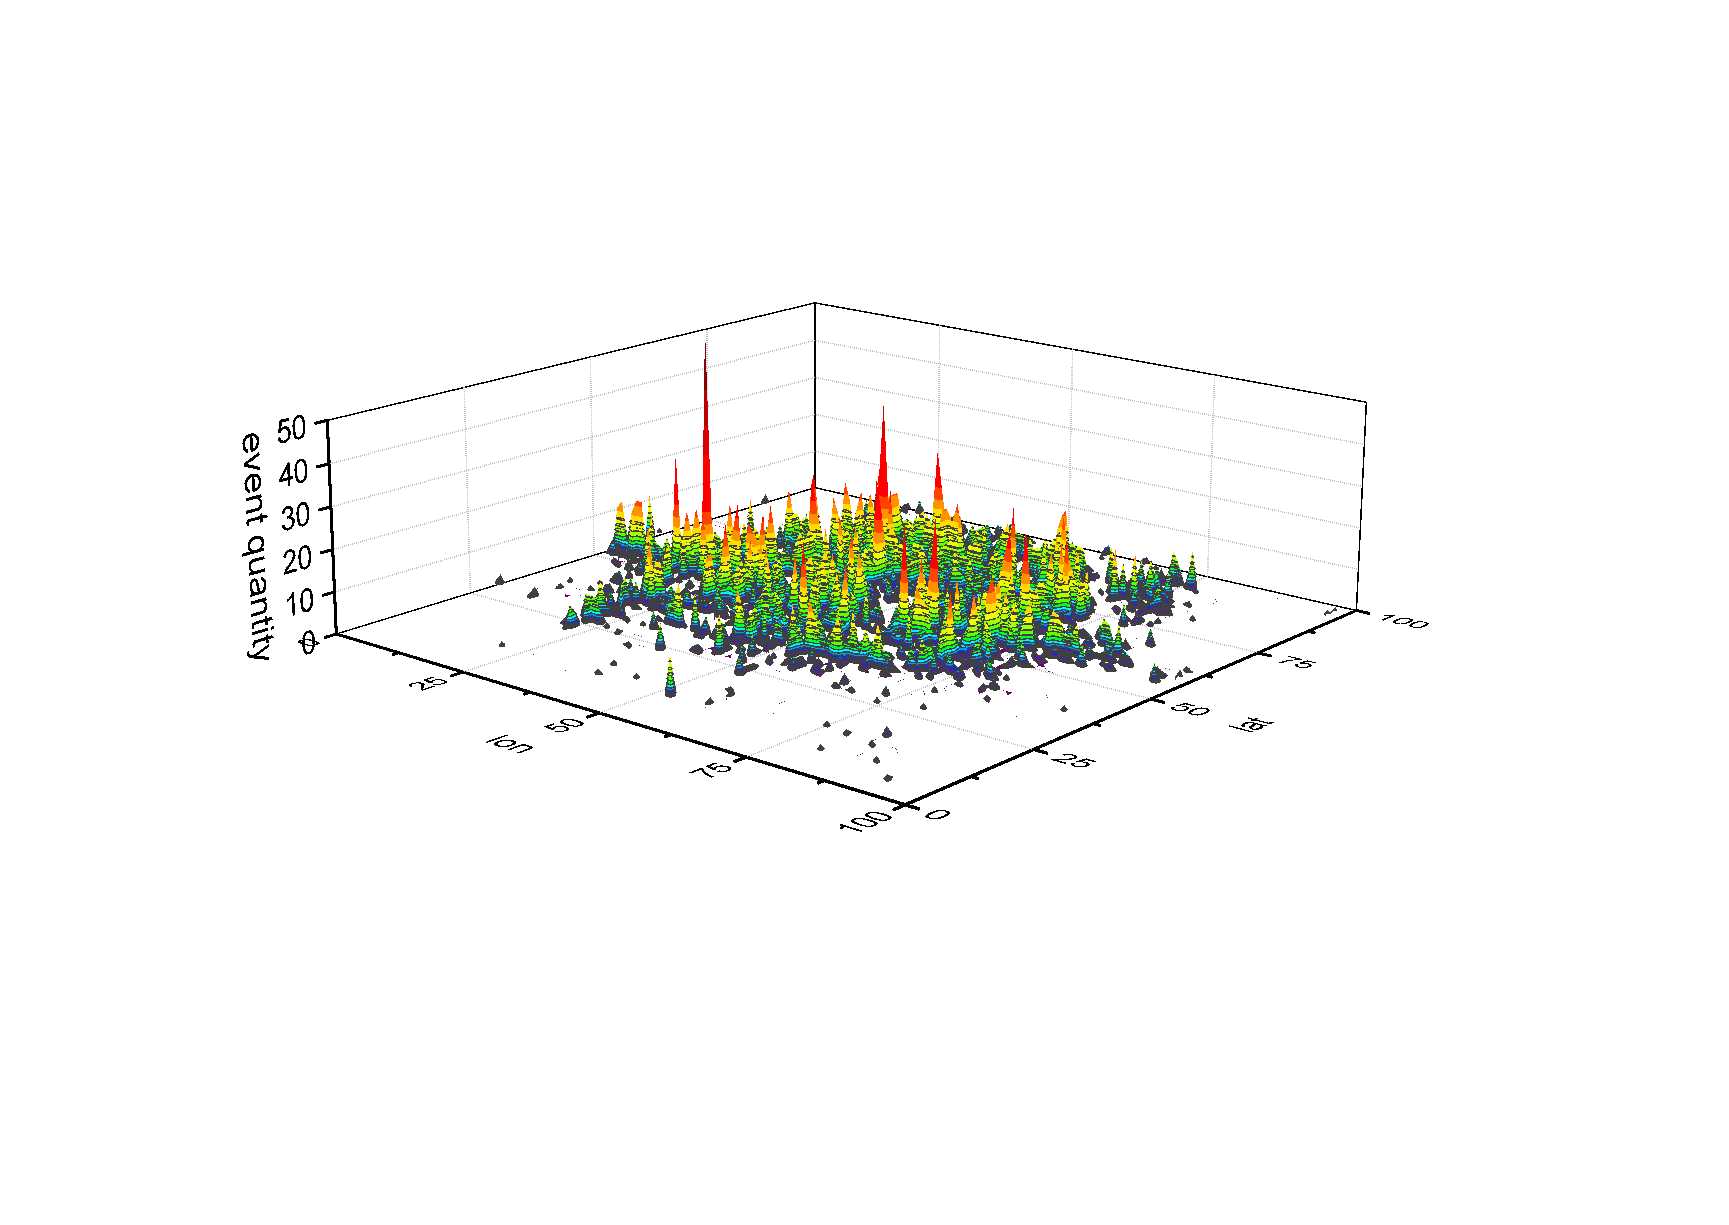
\includegraphics[width=0.23\textwidth]{figures_201103/events_dis/Graph6.eps}}
%\vspace{-0.14in}
%\subfigure[$drop,17:00-18:00$]{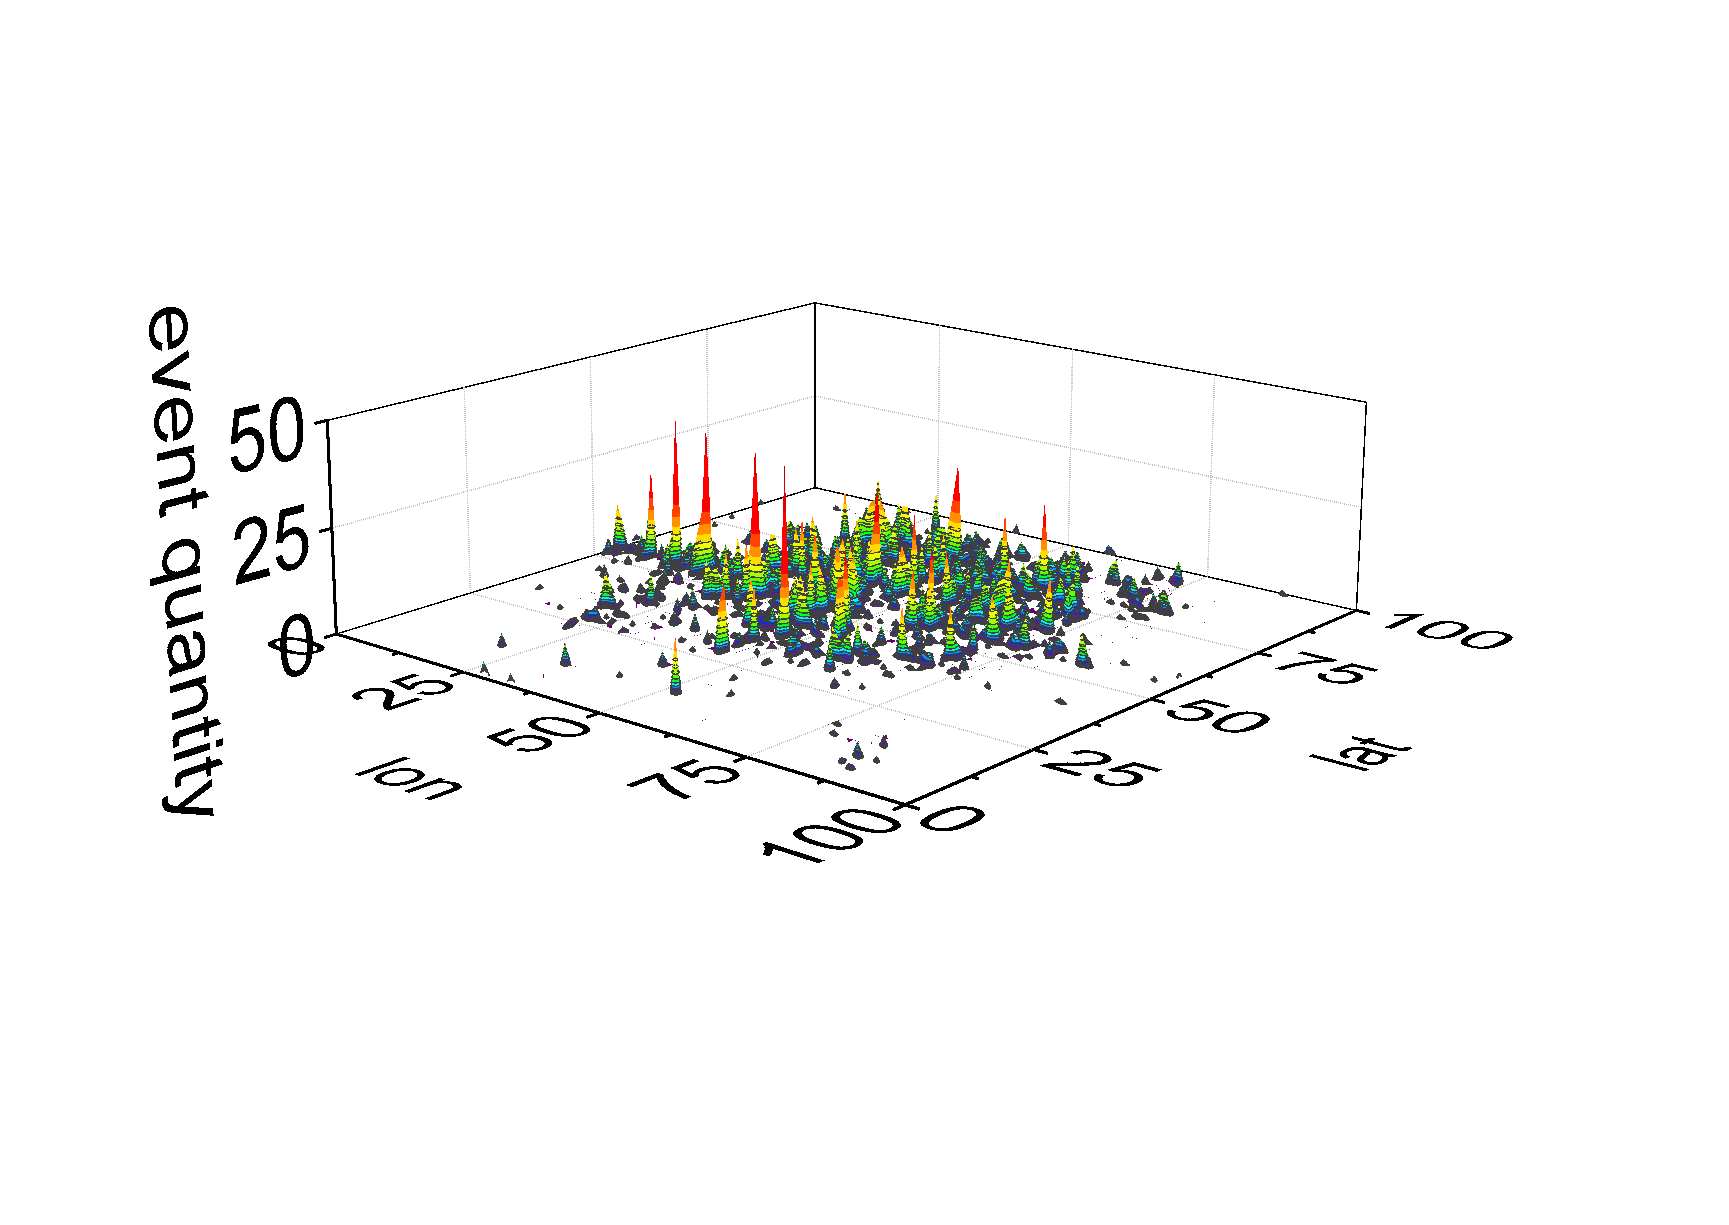
\includegraphics[width=0.23\textwidth]{figures_201103/events_dis/Graph3.eps}}
%\caption{Taxi density for load/drop events in one hour.}\label{figure_taxi_density_for_one_hour}
%\end{figure}


\begin{figure*}[!t]
\centering
\begin{tabular}
[c]{ccc}
\epsfysize=1.4in\epsfbox{figures_201103/events_dis/Graph4.eps} &
\epsfysize=1.4in\epsfbox{figures_201103/events_dis/Graph5.eps} &
\epsfysize=1.4in\epsfbox{figures_201103/events_dis/Graph6.eps} \\
(a) $load,7:00-8:00$ & (b) $load,12:00-13:00$ & (c) $load,17:00-18:00$\\
\epsfysize=1.4in\epsfbox{figures_201103/events_dis/Graph1.eps} &
\epsfysize=1.4in\epsfbox{figures_201103/events_dis/Graph2.eps} &
\epsfysize=1.4in\epsfbox{figures_201103/events_dis/Graph3.eps} \\
(d) $drop,7:00-8:00$ & (e) $drop,12:00-13:00$ & (f) $drop,17:00-18:00$
\end{tabular}
\caption{Taxi density for load/drop events in one hour.}\label{figure_taxi_density_for_one_hour}
\end{figure*}
